% =============================================================================
% FlashANNS --- ASPLOS 2027 September cycle (deadline 2026-09-09 AoE)
%
% REQUIRED class options (ASPLOS 2027 CFP):
%   sigplan, anonymous, review, nonacm
% Forbidden: \vspace squeezing, 9pt body, unnumbered pages.
% Limit: 11 pages of body+figures+tables; refs / appendix / AI ack free.
% Rapid Review: first TWO pages only. Keep §1 self-contained.
%
% 4.5/5 score bar this skeleton is written to:
%   Novelty     --- scoped "first graph-ANNS runtime on SSD-backed CXL VA"
%   Fit         --- OS residency + memory/storage hierarchy (two pillars)
%   Completeness--- Route A: opportunity + D1--D5 + DiskANN bakeoff + ablation
%   Honesty     --- proxy device, no 160 GB/s, Shared FAM is a model
%   Empirics    --- iso-recall, named cons, SIGPLAN-style disclosure (§5)
%   Presentation--- one claim per figure; money plot first in Eval
% =============================================================================
\documentclass[sigplan,anonymous,review,nonacm]{acmart}

\settopmatter{printfolios=true, printccs=true, printacmref=false}

\usepackage{booktabs}
\usepackage{graphicx}
\usepackage{tikz}
\usetikzlibrary{patterns}

% =============================================================================
% FlashANNS writing macros. Change the system name in one place.
% Numbers the authors have not yet locked go through \num{...}.
% =============================================================================
\newcommand{\sys}{FlashANNS}

% Fill-in numeric / qualitative result. Renders as a bold bracket so it cannot
% be mistaken for a measured number at submission time.
\newcommand{\num}[1]{[{\bfseries #1}]}

% Short inline "to be filled" token for table cells.
\newcommand{\ph}{\textemdash}

% -----------------------------------------------------------------------------
% Placeholder figure body. Caption is written by the caller and is the contract:
% when you replace the box, do not change what the caption claims unless the
% paper argument changes.
%   #1 width   (e.g. 0.98\columnwidth or 0.98\textwidth)
%   #2 height  (e.g. 3.4cm) -- keep modest; 11-page budget
%   #3 label shown inside the box (figure id + what to draw)
% -----------------------------------------------------------------------------
\newcommand{\phbox}[3]{%
  \begin{tikzpicture}
    \draw[thick, dashed, draw=black!45, fill=black!4]
      (0,0) rectangle (#1,#2);
    \node[align=center, text=black!55, font=\small,
          text width=0.92*#1] at (0.5*#1, 0.5*#2) {#3};
  \end{tikzpicture}%
}

% Common "fill later" footnote for tables.
\newcommand{\phnote}{Every \ph\ cell is a placeholder. Replace with the
  measured value under the protocol in~\S\ref{sec:eval-setup}.}


%% Clickable citations (ASPLOS CFP asks for this).
\hypersetup{colorlinks=true, citecolor=black, linkcolor=black, urlcolor=black}

\begin{document}

\title{FlashANNS: Hiding NAND from Graph Search on Flash-Backed CXL Memory}

\begin{abstract}
Billion-scale approximate nearest neighbor search (ANNS) must scale
corpus capacity and query throughput independently. Replicated block-SSD
systems such as DiskANN pay a storage-replication tax as query hosts
grow; full-in-memory CXL-DRAM systems such as CXL-ANNS and Cosmos pay a
DRAM-capacity tax on the cold tail. Flash-backed CXL memory (CXL-SSD)
is the third deployment point: a flash-priced corpus behind a small
memory-semantic window. The service we want is stronger than ``slightly
faster mmap'': from the host, scoring should look as if the working set
already lived in CXL-DRAM, while most of $D$ stays on CXL-SSD because
that window cannot hold the corpus. Prefetch, page admission, bandwidth
caps, and continuous batching exist to finish NAND fills
\emph{before} a hop scores---not to make a blocking miss cheaper.

We present \sys{}, a graph-ANNS runtime that treats a window miss on
the scoring path as a hide failure. Graph and PQ codes belong in host
DRAM so the window is 100\% vectors; only high-precision frontier pages
are admitted; search width is chosen at an iso-recall floor; fills are
issued asynchronously and batched across queries so one pointer-chasing
walk does not collapse device depth to one. The contract is 100\% of full-precision scores from the window and
DRAM-class critical-path wait: entry 2-hop is warmed off the timed
path, lookahead fills the next hop, and a miss while scoring is a
failure we close. Prior hop-ranked P3 on true-cold Text2Image-10M
(recall@10 $\ge 0.92$) was $3.3\times$ demand (5.35 vs.\ 1.64 QPS) with
only 3--34\% window hits---the gap the hide engine exists to remove.
A same-machine PipeANN block path remains the named residual. We evaluate an FPGA-attached
NVMe plus a software memory-semantic proxy (\texttt{vmem\_sw}), do not
claim a product CXL.mem SSD or a measured 160\,GB/s device-internal
path, and treat multi-host one-copy as a conditioned deployment model.
\end{abstract}

\begin{CCSXML}
<ccs2012>
 <concept>
  <concept_id>10010520.10010521.10010537</concept_id>
  <concept_desc>Computer systems organization~Secondary storage organization</concept_desc>
  <concept_significance>500</concept_significance>
 </concept>
 <concept>
  <concept_id>10002951.10002952.10003190.10003192</concept_id>
  <concept_desc>Information systems~Nearest-neighbor search</concept_desc>
  <concept_significance>500</concept_significance>
 </concept>
 <concept>
  <concept_id>10011007.10010940.10010971</concept_id>
  <concept_desc>Software and its engineering~Memory management</concept_desc>
  <concept_significance>300</concept_significance>
 </concept>
</ccs2012>
\end{CCSXML}

\ccsdesc[500]{Computer systems organization~Secondary storage organization}
\ccsdesc[500]{Information systems~Nearest-neighbor search}
\ccsdesc[300]{Software and its engineering~Memory management}

\keywords{CXL, CXL-SSD, approximate nearest neighbor search, graph ANNS,
  memory-semantic flash, residency, prefetch, continuous batching}

\maketitle

% =============================================================================
% §1 Introduction  — Rapid Review lives or dies here (first two pages).
% Target: 1.8--2.0 pages including Fig.~1 and the contribution list.
% 4.5/5 bar: problem is ASPLOS (OS residency + memory/storage hierarchy),
% novelty is scoped, contributions are falsifiable, first two pages self-contained.
% 填写: 把 \num{...} 换成终表数字；替换 Fig.~1 框图；不要改贡献句的范围。
% =============================================================================
\section{Introduction}
\label{sec:intro}

Billion-scale approximate nearest neighbor search (ANNS) must scale two
\emph{independent} dimensions: \emph{corpus capacity} and \emph{query
throughput}. Adding query hosts does not, by itself, shrink the full-precision
graph and embedding store; growing that store does not, by itself, create more
CPU and I/O. Production serving therefore faces a deployment question that
neither ``use a better graph'' nor ``buy a faster SSD'' answers:

\begin{quote}
\emph{When query load grows, can we add compute without replicating the cold
corpus, and without lifting that corpus into DRAM-priced memory?}
\end{quote}

Two published deployment points dominate the literature, and each taxes one
of those dimensions. Block-SSD graph systems such as
DiskANN~\cite{diskann,freshdiskann} and its pipelined descendants~\cite{pipeann}
are excellent at hiding NAND latency behind asynchronous block I/O, product
quantization (PQ) navigation, and a per-host node cache. Their common serving
unit, however, is still \emph{CPU $+$ DRAM working set $+$ a local SSD index}.
Scaling throughput by $R$ query workers therefore typically
replicates provisioned flash ($\propto R\cdot D$) or shards the graph and pays
cross-shard fan-out. Remote block access (NVMe-oF) moves the cable, not the
tax: each host still maintains its own page/buffer cache. Distributed
serving~\cite{distributedann} shows that a single logical DiskANN graph can
live behind a shared KV store, but the interface remains block/KV, not a
unified load/store address space.

The complementary point is full-in-memory CXL-DRAM ANNS.
CXL-ANNS~\cite{cxlanns,cxlanns-tocs} and Cosmos~\cite{cosmos} put the graph
and embeddings in a CXL memory pool so that search never stalls on flash.
That design eliminates NAND misses, and a pooled HDM \emph{can} be one copy
--- but it prices the \emph{cold tail} at DRAM. For a corpus of size $D$ whose
hot working set $H$ satisfies $H\ll D$, the stranded-capacity problem is
structural~\cite{bauhaus,secondtier}: most vectors are rarely touched and
still occupy a DRAM-class device.

Flash-backed CXL memory (CXL-SSD) is the missing third point
(Figure~\ref{fig:intro-position}). A Type-3 memory-semantic SSD exposes NAND
capacity and a small device/host DRAM window through \texttt{load}/\texttt{store}
on a CXL.mem address space~\cite{skybyte,fromblocktobyte,cmm-h,cxl30}. Relative
to replicated DiskANN, the opportunity is to stop copying $D$ with every added
query host; relative to CXL-ANNS/Cosmos, it is to price the cold corpus at
flash. Under CXL 3.x Shared FAM/GFAM, multiple hosts can map the same region
concurrently~\cite{cxl30} --- a \emph{deployment} path to one-copy serving, not
a mechanism we claim to have evaluated. We state the three CXL conditions
explicitly so they are not conflated: (i)~direct-attach CXL-SSD already
provides flash-priced memory semantics on one host; (ii)~CXL 2.0 pooling
shares a device, not a concurrently mapped HDM region; (iii)~only Shared FAM
is a standard premise for multi-host one-copy.

\begin{figure*}[t]
  \centering
  \phbox{0.98\textwidth}{3.6cm}{%
    Fig.~1 placeholder --- draw three columns:\\
    (a)~replicated local-SSD DiskANN ($R\times D$ flash, per-host cache);\\
    (b)~full-in-memory CXL-DRAM ANNS ($D$ at DRAM price);\\
    (c)~\sys{}: graph/PQ in host DRAM, hot records in a bounded CXL-DRAM
    window, full-precision corpus on CXL-SSD, optional Shared-FAM caption.}
  \caption{Three deployment points for billion-scale graph ANNS, and the
    \sys{} runtime that sits on the third. CXL-SSD is an \emph{opportunity}
    (flash-priced corpus, memory-semantic hot path, one-copy under Shared FAM).
    The \emph{system} is residency and stall control on that tier.
    \textbf{Fill-in:} replace this box with a 3-column deployment drawing plus
    a compact runtime overlay on (c). Do not draw a 160\,GB/s device-internal
    bus as a measured link.}
  \Description{Three-column comparison of replicated SSD ANNS, full CXL-DRAM
    ANNS, and the proposed flash-backed CXL-SSD system.}
  \label{fig:intro-position}
\end{figure*}

CXL-SSD does \emph{not} make NAND as fast as DRAM. A cold vector load on this
tier costs tens of microseconds --- two orders of magnitude above a CXL-DRAM
or host-DRAM hit (Figure~\ref{fig:mot-cliff}). Treating the device as slightly
slow memory, or as ``mmap DiskANN'', fails in four systematic ways that we
measure in~\S\ref{sec:motivation}: (1)~the miss cliff dominates end-to-end
search once any material fraction of loads miss; (2)~OS-style page admission
is a poor match for high-dimensional graph adjacency and inflates NAND reads;
(3)~synchronous or high-coverage graph prefetch pollutes the small DRAM window
and can \emph{reduce} QPS; (4)~a blocking load/store miss collapses device
queue depth to $\approx 1$, so a scheduler designed for \texttt{io\_uring}
depth can become a pessimization until fills are made asynchronous. Widening
search (\texttt{efSearch} / beam) to ``buy recall'' further cools the working
set and couples quality to stall.

This paper presents \sys{}, a graph-ANNS \emph{runtime} whose service
goal is to make CXL-SSD \emph{invisible on the search critical path}.
The host should score as if the working set already lived in a small
CXL-DRAM window; the corpus stays on flash because that window cannot
hold $D$. Prefetch, page admission, bandwidth caps, and continuous
batching exist to finish NAND fills \emph{before} a hop scores---not to
make blocking \texttt{load}/\texttt{store} slightly faster.
\sys{} does not replace DiskANN's block-SSD path and does not assume
the corpus fits in CXL-DRAM. A single walk cannot hide hop $i{+}1$
until hop $i$ scores (pointer-chasing); inter-query continuous issue is
what keeps device depth up while one walk is stuck.
The runtime has five coupled modules
(\S\ref{sec:design}): semantic placement; bounded window admission;
entry / soft-pin (not a thrashing LFU hot set); stall-aware search
control; and continuous fetch-level batching over asynchronous
memory-semantic reads.

To our knowledge, this is the first \emph{graph-ANNS serving system} that
directly operates over an SSD-backed CXL address space and jointly manages
ANNS-specific residency, promotion, and search stalls. We do \emph{not} claim
to be the first work to attach a CXL-SSD to a vector database, nor that we
have deployed Shared FAM in production.

This paper makes four contributions:

\begin{enumerate}
  \item \textbf{A third deployment point, stated with its limits.} We
    separate the CXL-SSD \emph{opportunity} (flash-priced $D$, a small
    memory-semantic window, optional one-copy) from the \emph{system}
    (hide NAND from the ANNS critical path), and we name
    the CXL 2.0 vs.\ 3.x conditions under which one-copy is even
    well-formed~(\S\ref{sec:intro}, \S\ref{sec:background}).
  \item \textbf{A measured pathology of graph ANNS on this tier.} We show
    that naive page caches, blind prefetch, unconstrained search width, and
    blocking load/store each amplify stall, and we turn the negative results
    into design constraints~(\S\ref{sec:motivation}).
  \item \textbf{A runtime that tries to hide flash from graph search.}
    \sys{} places graph/PQ off the window, admits few pages, prefetches
    the next hop off the scoring path, and batches fills across queries
    under an iso-recall $L$~(\S\ref{sec:design}, \S\ref{sec:impl}).
  \item \textbf{An iso-recall evaluation of hide, not just QPS.}
    At matched recall we report critical-path wait, window-hit on scored
    vectors, QPS vs.\ demand and vs.\ an in-window oracle, and a
    same-machine DiskANN/PipeANN residual~(\S\ref{sec:eval}).
\end{enumerate}

\paragraph{Scope we do not claim.}
The prototype is an FPGA Type-2/BAR endpoint (\texttt{mem2nvme}/\texttt{nvmex})
plus a software memory-semantic node (\texttt{/dev/vmem0}, \texttt{vmem\_sw})
in front of a 1.92\,TB NVMe. Device HPS and CPU writes into the 32\,GiB BAR
are not live; we do not publish BAR-path numbers. A Montage-style CXL-DRAM
DAX window is \emph{absent} on the measured boot---the 1\,GiB search window
is host DRAM (\texttt{mbind}). We do not report 160\,GB/s device-side copy,
product CXL.mem SSD, or Shared-FAM one-copy. Cost claims are qualitative.

The rest of the paper is organized as follows.
\S\ref{sec:background} reviews graph ANNS and CXL memory-semantic flash.
\S\ref{sec:motivation} presents the findings that constrain the design.
\S\ref{sec:design}--\S\ref{sec:impl} describe \sys{}.
\S\ref{sec:eval} evaluates it.
\S\ref{sec:related} and~\S\ref{sec:discuss} place the work and state limits.

% =============================================================================
% §2 Background  — Target: 0.8--1.0 page. No new claims.
% 4.5/5 bar: enough for a non-ANNS ASPLOS reviewer to follow Design/Eval;
% every compared system is named with its medium and interface.
% 填写: 补 CXL-SSD 设备框图（Fig.~2）上的真实端口/窗口数字。
% =============================================================================
\section{Background and Deployment Points}
\label{sec:background}

\subsection{Graph ANNS and the block-SSD path}
\label{sec:bg-anns}

A graph ANNS index (Vamana~\cite{diskann}, HNSW~\cite{hnsw}) stores, for each
vector, a small neighbor list. Search maintains a candidate set of width
$L$ (beam / \texttt{efSearch}), repeatedly expanding the closest unread node,
and returns the top-$k$. Quality is monotone in how many nodes are scored;
\emph{stall} is monotone in how many of those scores miss the fast tier.

DiskANN~\cite{diskann,freshdiskann} is the reference block-SSD design. Full-
precision vectors and adjacency live in 4\,KB-aligned sectors on NVMe. A
compact PQ codebook in DRAM scores neighbors without a NAND read; an
\texttt{aio} beam issues several sector reads at once; a static node cache
pins entry vertices. PipeANN~\cite{pipeann} keeps that layout and overlaps
compute with I/O inside a single query, and can interleave queries to raise
device queue depth. The first-class objects of this path are \emph{the I/O
queue and the sector}. They are the wrong first-class objects once the
device is no longer a block target but a faulting address space
(\S\ref{sec:motivation}).

\subsection{CXL-DRAM ANNS}
\label{sec:bg-cxl-dram}

CXL.mem lets a host map device HDM into its physical address space~\cite{cxl30}.
CXL-ANNS~\cite{cxlanns,cxlanns-tocs} places the essential graph and embeddings
in a Type-3 CXL-DRAM pool and hides $\sim$100\,ns far-memory delay with a
relationship-aware cache and DSA-assisted prefetch. Cosmos~\cite{cosmos}
further offloads traversal and distance to device-side compute. Second-tier
and residual-quantization designs~\cite{secondtier,fatrq,hm-ann} also assume
a DRAM- or NVM-priced far tier. \sys{} shares the \emph{interface}
(load/store) with this line and rejects its \emph{capacity assumption}
(the corpus fits in CXL-DRAM).

\subsection{Flash-backed CXL memory}
\label{sec:bg-cxl-ssd}

A CXL-SSD pairs NAND with a modest DRAM cache and presents a byte-addressable
window~\cite{skybyte,fromblocktobyte,cmm-h}. A hit is a CXL.mem load; a miss
is a NAND fill into that window, then a retry. The programming model looks
like memory; the miss tax looks like flash. Hardware and generic OS work on
this tier does not manage graph-ANNS residency. CXL-AnySSD~\cite{cxl-anyssd}
accelerates vector-DB traffic by removing swap, not by controlling promote
precision or search stalls. P-HNSW~\cite{phnsw} studies crash-consistent
graphs and mentions CXL-SSD; its experiments use DRAM-simulated PM.

Three conditions must not be mixed when we talk about sharing
(Figure~\ref{fig:bg-cxl}):

\begin{enumerate}
  \item \textbf{Direct-attach CXL-SSD.} One host, flash price, memory
    semantics. Sufficient for the single-host claims in this paper.
  \item \textbf{CXL 2.0 pooling / MLD.} Several hosts may time-share a
    device; a given HDM region is owned by one host at a time.
  \item \textbf{CXL 3.x Shared FAM / GFAM.} Several hosts may map the same
    region at once. This is the standard premise for multi-host one-copy
    serving, and additionally requires a fabric manager and a read-only
    publish protocol. We do not evaluate it.
\end{enumerate}

\begin{figure}[t]
  \centering
  \phbox{0.98\columnwidth}{3.2cm}{%
    Fig.~2 placeholder --- CXL-SSD stack:\\
    host CPU $\rightarrow$ CXL link $\rightarrow$ endpoint
    (DRAM window $+$ FTL $+$ NAND).\\
    Annotate: host-side link is per-host; device-side bandwidth is shared.}
  \caption{Flash-backed CXL memory. Host-side CXL links are independent;
    device-side port, controller, DRAM cache, FTL, and NAND are shared.
    One-copy reduces replicated capacity; it does not replicate SSD IOPS.
    \textbf{Fill-in:} use the real endpoint you measure; mark the software
    proxy path if that is the prototype.}
  \Description{Block diagram of a host attached to a CXL-SSD endpoint with
    a small DRAM window in front of NAND.}
  \label{fig:bg-cxl}
\end{figure}

\paragraph{Media-cost sketch (qualitative).}
Let $c_{\mathrm{DRAM}}$ and $c_{\mathrm{flash}}$ be unit media prices and
$n_{\mathrm{HA}}$ the number of high-availability copies ($n_{\mathrm{HA}}\ll R$
in the common case). Then
\[
  \mathrm{MediaCost}_{\text{CXL-DRAM}} \sim D\cdot c_{\mathrm{DRAM}},
\]
\[
  \mathrm{MediaCost}_{\text{CXL-SSD}} \sim n_{\mathrm{HA}} D\cdot c_{\mathrm{flash}}
    + H\cdot c_{\mathrm{cache}} + C_{\mathrm{fabric}}.
\]
We use this only to locate the third deployment point
(Figure~\ref{fig:eval-scale}). We do not claim a lower TCO.

% =============================================================================
% §3 Motivation  — Target: 1.4--1.6 pages. Every finding is (A) exists (B) hurts.
% 4.5/5 bar: negative results become design constraints, not embarrassment.
% 填写: 换 Fig.~3--5 和 Table~1 的实测；caption 里的定性结论不要改，除非 finding 变了。
% =============================================================================
\section{Why Naive CXL-SSD ANNS Fails}
\label{sec:motivation}

A unified VA does not make graph ANNS fast. This section records the
pathologies that a runtime must treat as first-class. Each finding answers
two questions: \emph{does the effect exist in the numbers?} and \emph{how
much does being wrong cost?} We later require every design module to name
the finding it answers (Table~\ref{tab:findings}).

\subsection{F1: A two-order miss cliff}
\label{sec:mot-cliff}

A full-precision load that misses the CXL-SSD window costs
tens of microseconds on the measured path (true-cold mean promote
24--72\,$\mu$s; Figure~\ref{fig:mot-cliff}). A hit that is already in
the 1\,GiB window is a host memcpy (sub-microsecond). The ratio is two
orders of magnitude. Graph search multiplies this tax by hops
$\times$ degree. Once a modest fraction of loads miss, wall-clock time is
spent in the NAND path, not in distance arithmetic. DiskANN already knew
this for block I/O; the new fact is that \emph{memory-semantic} access does
not remove the cliff --- it only changes how a miss is issued
(\S\ref{sec:mot-qd}).

\begin{figure}[t]
  \centering
  \phbox{0.98\columnwidth}{3.3cm}{%
    Fig.~3 placeholder --- three bars or a CDF:\\
    cold NAND / soft-cache$+$PTE-cold / PTE-warm.\\
    Optional stacked bar: fraction of a full search in each tier.}
  \caption{Miss cliff on flash-backed CXL memory. Soft-cache hits are
    \emph{not} PTE hits; reporting only \texttt{mincore}/PTE occupancy
    hides the middle step. \textbf{Fill-in:} per-vector latency and a
    whole-search breakdown on the same index.}
  \Description{Bar chart of vector-load latency at three residency tiers.}
  \label{fig:mot-cliff}
\end{figure}

\subsection{F2: Page admission mismatches the graph}
\label{sec:mot-page}

Neighbor IDs are not sequential in the address space. Admitting 16\,KB OS
pages (or CXL-SSD cachelines grouped as pages) therefore brings vectors the
search will not score. On a high-dimensional corpus where a vector is
already close to a page, page admission versus per-record admission
splits QPS by \num{$\sim$3.6$\times$} and NAND reads by
\num{$\sim$3.7$\times$} (Figure~\ref{fig:mot-pathology}a). The claim is
scoped: at small dimensions several records share a page and the gap
narrows. Default page-cache thinking is still the wrong default for this
workload.

\subsection{F3: Promotion volume without precision is harmful}
\label{sec:mot-pref}

Synchronous logical prefetch of 1-, 2-, or 8-hop neighborhoods leaves
hit rate almost unchanged, multiplies NAND reads, and drops QPS by
\num{$\sim$4--5$\times$} at the widest setting
(Figure~\ref{fig:mot-pathology}b). Precision (\emph{used$/$promoted})
falls as coverage grows; leftover pages evict useful ones from a
few-gigabyte window. \emph{Wrong promotion costs more than a missed
promotion.} The useful policy is a bounded, high-precision ensure of the
nodes the search is about to expand --- not ``prefetch harder.''

\subsection{F4: Search width is a stall knob}
\label{sec:mot-beam}

Raising \texttt{efSearch} / beam grows the unique IDs touched per query,
cools the window, and raises NAND reads faster than it raises recall
(Figure~\ref{fig:mot-pathology}c). Recall itself saturates once a hop
budget is spent. A shared hot set at a \emph{small} beam beats a cold
cache at a \emph{large} beam. A controller that chops beam on instantaneous
miss rate does not, by itself, win at iso-recall: it has no recall
constraint and no IO budget. Quality and stall must be controlled jointly.

\begin{figure*}[t]
  \centering
  \phbox{0.98\textwidth}{3.5cm}{%
    Fig.~4 placeholder --- three panels, same y-family (QPS or normalized):\\
    (a)~record vs.\ 16\,KB page admission;\\
    (b)~demand vs.\ 1-/2-/8-hop sync prefetch (precision annotated);\\
    (c)~efSearch / beam sweep: QPS, hit\%, recall@10, NAND reads.}
  \caption{Three default usages that amplify stall. (a)~Page admission.
    (b)~Blind graph prefetch. (c)~Widening search. Each panel must keep
    recall visible so raw QPS cannot be misread.
    \textbf{Fill-in:} one protocol (dataset, $L$, cache bytes) across
    panels if possible.}
  \Description{Three-panel figure of page admission, prefetch precision,
    and search-width coupling.}
  \label{fig:mot-pathology}
\end{figure*}

\subsection{F5: A single query cannot fill the miss pipeline}
\label{sec:mot-qd}

Graph search is pointer-chasing. Even an excellent single-query pipeline
leaves device-queue bubbles: the next hop is unknown until the current
page is scored, the beam ramps slowly, and the query drains at the end
(Figure~\ref{fig:mot-bubbles}). On NVMe, interleaving independent queries
raises occupancy; a \emph{continuous}, fetch-level scheduler that admits
work at read granularity can hold a target depth $D$.

On CXL-SSD the same idea is necessary and insufficient. A blocking
\texttt{memcpy} from a mapping is a synchronous NAND fault (effective
QD$\approx 1$ per thread). A depth-oriented scheduler that issues
\emph{speculative} fills then pays their latency on the critical path and
can lose to a narrower pipeline. Continuous batching pays off on this tier
only after memory-semantic fills are asynchronous
(Figure~\ref{fig:design-pipe}, \S\ref{sec:d4}).

\begin{figure}[t]
  \centering
  \phbox{0.98\columnwidth}{3.4cm}{%
    Fig.~5 placeholder --- in-flight depth vs.\ time:\\
    (a)~single-query pipeline; (b)~static batch; (c)~continuous fetch batching.\\
    (Existing TikZ in sections/fig\_bubbles.tex can replace this box.)}
  \caption{Pipeline bubbles. $y$ is in-flight device reads; $D$ is the
    depth needed to exercise NAND parallelism. A single query cannot hold
    $D$; a static batch drains at the barrier; continuous fetch-level
    admission targets $D$ at unchanged recall.
    \textbf{Fill-in:} swap in the measured schematic; add a CXL-SSD panel
    that shows blocking load/store stuck at QD$\approx 1$.}
  \Description{Three timelines of device queue occupancy under different
    schedulers.}
  \label{fig:mot-bubbles}
\end{figure}

\subsection{From findings to design constraints}
\label{sec:mot-map}

Table~\ref{tab:findings} is the contract for~\S\ref{sec:design}. We do not
treat CXL-SSD as uniform memory (C1). We place the graph and PQ off the
SSD window (C2). We promote few, precise records (C3) and share them
across queries (C4). We control beam under iso-recall or an IO budget
(C5), and we issue misses asynchronously at a target depth. Evaluation
must compare against a block-SSD path on the same corpus and recall
(C6).

\begin{table}[t]
  \caption{Findings become challenges become knobs.
    \textbf{Fill-in:} replace \ph\ with the headline measured delta
    (e.g., QPS $\times$, IO $\times$).}
  \label{tab:findings}
  \small
  \begin{tabular}{@{}p{0.07\columnwidth}p{0.28\columnwidth}p{0.26\columnwidth}p{0.27\columnwidth}@{}}
    \toprule
    ID & Finding (exists $+$ hurts) & Challenge & \sys{} knob \\
    \midrule
    F1 & Miss cliff \ph$\times$ & C1 visibility of tiers & counters, cost model \\
    F2 & Page $\neq$ record \ph$\times$ & C2 placement & record / hub admission \\
    F3 & Low-precision promote \ph$\times$ & C3 bounded promote & top-$M$, byte budget \\
    F4 & Beam cools the set \ph & C5 iso-recall & beam / early stop \\
    F5 & Bubbles; mmap QD$\approx 1$ & C4/C5 pipeline & async fill $+$ \texttt{cont} \\
    F7 & Shared hot set $>$ deep beam & C4 shared cache & cross-query pin \\
    \bottomrule
  \end{tabular}\\[2pt]
  {\footnotesize \phnote}
\end{table}

% =============================================================================
% §4 Design  — Route A: all five modules. Target: 2.5--2.8 pages.
% 4.5/5 bar: each module names the finding it answers; interfaces are concrete;
% what is forbidden is as clear as what is done.
% 填写: 换 Fig.~6--8；补 API 名字与真实阈值；不要新增第六个“也做了”的模块。
% =============================================================================
\section{Design}
\label{sec:design}

\sys{} is a userspace ANNS runtime plus a thin residency plane in front of host DRAM, a bounded window that plays the role of CXL-DRAM, and a flash-backed CXL address space that holds $D$ (Figure~\ref{fig:design-arch}).
Search is still best-first graph walk.
The service contract is a \emph{split}: prefetch and continuous batching may touch CXL-SSD; the scoring thread may not.
A hop that computes a full-precision distance from bytes that were not already in the window is a hide failure, not a successful promote.

The wise prefetcher turns a committed PQ rerank set into one precise page batch before full-precision scoring.
That precision does not remove the query's materialization barrier: its rerank still waits for its own batch.
Continuous batching exploits the independence across queries to cover that wait with other useful work.
The modules below separate these two roles and the evaluation tests them independently.

\begin{figure*}[t]
  \centering
  \phbox{0.98\textwidth}{3.8cm}{%
    Fig.~6 placeholder --- architecture:\\
    top: Placement $|$ Window admit $|$ Prefetch+\texttt{cont} $|$ $L$ ctrl;\\
    middle: residency plane (fill off crit path / score from window);\\
    bottom: host DRAM (graph/PQ) $|$ window $=$ virtual CXL-DRAM $|$ CXL-SSD.}
  \caption{\sys{} architecture.
    From the host, scored bytes look like CXL-DRAM; capacity is CXL-SSD.
    The residency plane is the only path that moves full-precision bytes.
    Search never page-faults a neighbor ``to be helpful.''
    \textbf{Fill-in:} use shipped names (\texttt{PREFETCH\_BATCH}, DramWindow); mark \texttt{vmem\_sw}.}
  \Description{Layered architecture of the ANNS runtime over three memory tiers.}
  \label{fig:design-arch}
\end{figure*}

\subsection{D1: Semantic placement}
\label{sec:d1}

Table~\ref{tab:placement} is the default map.
The graph adjacency and the PQ codebook are touched on every hop and are small relative to the full-precision corpus; they live in host DRAM so they never compete with vectors for the CXL-SSD window (F2, F7).
Query state (candidates, visited set, thread-local arenas) is likewise host-local.
Full-precision vectors default to the CXL-SSD address space.
A bounded \emph{hub / shared hot set} of vector pages is explicitly cached into the window or into CXL-DRAM (\S\ref{sec:d3}).
Only full-precision vectors in a committed rerank set become prefetch candidates; a discovered frontier does not (F3).

This is a deliberate difference from DiskANN, where adjacency and vectors share SSD sectors.
We pay a modest host-DRAM tax for the graph in order to stop the window from turning into an accidental adjacency cache.

\begin{table}[t]
  \caption{Default placement. \textbf{Fill-in:} bytes on the corpus you report (e.g., 25M $\times$ dim).}
  \label{tab:placement}
  \small
  \begin{tabular}{@{}p{0.28\columnwidth}p{0.22\columnwidth}p{0.42\columnwidth}@{}}
    \toprule
    Object & Default tier & Why \\
    \midrule
    Graph ($R$ neighbors) & host DRAM & every hop; keep off the window \\
    PQ / codebook        & host DRAM & tiny, extremely hot \\
    Query / visited      & host DRAM & per-worker state \\
    Full-precision vec.  & CXL-SSD   & capacity \\
    Entry / soft-pin     & window (tiny) & F7; LFU hot set demoted \\
    Committed rerank vec. & window via prefetch & F3, F5; score only if resident \\
    \bottomrule
  \end{tabular}
\end{table}

\subsection{D2: Wise prefetch at candidate commitment}
\label{sec:d2}

\paragraph{When: after commitment.}
The host first completes its approximate beam using the adjacency graph and PQ codes, without reading full-precision vectors from Flash.
When that beam commits the bounded rerank set $C_L$, the prefetcher issues immediately: after uncertainty has been pruned, but before exact scoring dereferences any vector in $C_L$.
This trigger deliberately gives up speculative lead time to avoid moving payload for candidates that will not survive.
The single-query path may still wait for materialization to complete; the invariant is that the subsequent scoring loads do not themselves fault on Flash.

\paragraph{What: the committed payload.}
The residency plane maps the IDs in $C_L$ to their full-precision vector pages, removes pages that are resident or already in flight, and deduplicates the rest.
Every requested page is therefore justified by at least one vector that exact reranking will consume.
Adjacency, PQ codes, speculative neighbors, and unused frontier records are not part of this wave.
Because Flash moves 4\,KiB pages, however, a justified page may still carry vector slots that this query will not score.

\paragraph{How: make each page useful.}
Offline, a co-use-aware layout groups vectors that disjoint training searches tend to request together and places the resulting pages into short runs.
Online, exact page filtering avoids duplicate movement, and the runtime fills gaps only in a short, sufficiently dense run; it never expands a sparse request into a whole SSD stripe.
This combination targets useful payload per read rather than batch size alone.
Unlike generic remote-memory or device-side sequential prefetchers~\cite{leap,cacheinhand}, the request is justified by the committed rerank set rather than an inferred address stream.
We distinguish page precision (a fetched page contains any scored vector), vector-slot utilization (scored slots over all slots read), and extent utilization (requested pages over pages transferred after coalescing); vector-slot utilization is the direct measure of real in-page use.

\begin{figure}[t]
  \centering
  \resizebox{0.88\columnwidth}{!}{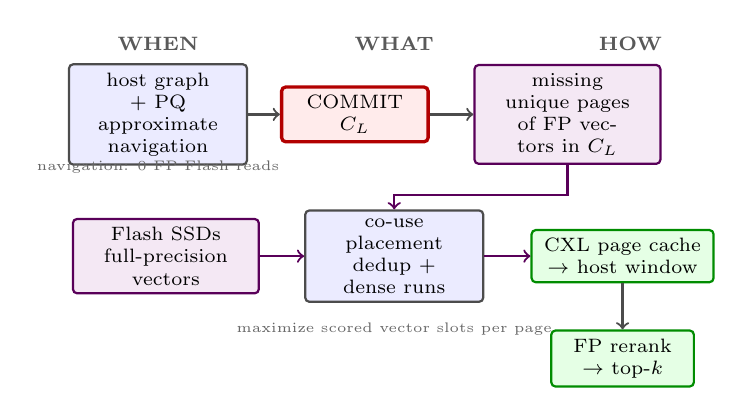
\begin{tikzpicture}[
  x=1cm,y=1cm,
  box/.style={draw=black!70, rounded corners=1.5pt, thick,
              align=center, inner sep=3pt, font=\scriptsize},
  info/.style={box, fill=blue!8},
  commit/.style={box, draw=red!70!black, fill=red!8, very thick},
  payload/.style={box, fill=violet!9, draw=violet!70!black},
  resident/.style={box, fill=green!10, draw=green!55!black},
  flow/.style={->, thick, draw=black!70},
  data/.style={->, thick, draw=violet!70!black},
  label/.style={font=\scriptsize\bfseries, text=black!65}
]
  \node[label] at (1.15,4.25) {WHEN};
  \node[label] at (4.15,4.25) {WHAT};
  \node[label] at (7.15,4.25) {HOW};

  \node[info,text width=2.05cm] (pq) at (1.15,3.35)
    {host graph + PQ\\approximate navigation};
  \node[commit,text width=1.65cm] (commit) at (3.65,3.35)
    {COMMIT\\$C_L$};
  \node[payload,text width=2.15cm] (select) at (6.35,3.35)
    {missing unique pages\\of FP vectors in $C_L$};
  \draw[flow] (pq)--(commit);
  \draw[flow] (commit)--(select);
  \node[font=\tiny,text=black!60,align=center] at (1.15,2.68)
    {navigation: 0 FP Flash reads};

  \node[payload,text width=2.15cm] (flash) at (1.25,1.55)
    {Flash SSDs\\full-precision vectors};
  \node[info,text width=2.05cm] (shape) at (4.15,1.55)
    {co-use placement\\dedup + dense runs};
  \node[resident,text width=2.10cm] (window) at (7.05,1.55)
    {CXL page cache\\$\rightarrow$ host window};
  \node[resident,text width=1.60cm] (rerank) at (7.05,0.25)
    {FP rerank\\$\rightarrow$ top-$k$};

  \draw[data] (select.south) -- ++(0,-0.38) -| (shape.north);
  \draw[data] (flash)--(shape);
  \draw[data] (shape)--(window);
  \draw[flow] (window)--(rerank);

  \node[font=\tiny,text=black!60,align=center] at (4.15,0.62)
    {maximize scored vector slots per page};
\end{tikzpicture}
}
  \caption{Wise prefetch answers three questions.
    \emph{When}: after PQ navigation commits $C_L$.
    \emph{What}: only missing unique pages of its full-precision vectors.
    \emph{How}: co-use-aware placement, exact filtering, and dense short runs increase useful vector slots per Flash read.}
  \Description{A left-to-right pipeline showing PQ candidate commitment, selection of missing full-precision vector pages, locality-aware request formation, materialization into the CXL cache and host window, and exact reranking.}
  \label{fig:design-promote}
\end{figure}

\subsection{D3: Entry pin and soft-pin (hot set demoted)}
\label{sec:d3}

Single-query deepening is a bad way to spend a small window (F4, F7).
A 64\,MiB shared LFU set raised hit rate and \emph{destroyed} QPS on a warm protocol (14.3$\rightarrow$2.4); we do not ship it as D3.
What remains is a tiny hard pin of the entry subgraph ($\le$32\,MiB) and a hop-decaying soft-pin of recently installed pages.
Pinning is never implicit in a page fault.
Cross-query reuse, if it happens, is because committed materialization left useful pages in the window---not because an LFU daemon is competing with search.

\subsection{D4: Hide engine --- wise prefetch and continuous batching}
\label{sec:d4}

\paragraph{A query-local barrier.}
D2 creates one precise materialization wave after PQ navigation commits $C_L$,
but the same query cannot rerank until that wave completes.
Better page selection alone therefore cannot keep Flash busy.

\paragraph{Cross-query overlap.}
The barrier is local to a query, not to the service: while one query waits,
another can navigate, materialize its own committed wave, or rerank resident
bytes.
Continuous batching interleaves these stages so host work and Flash access
coexist (Figure~\ref{fig:design-pipe}).
Like continuous scheduling in other staged serving systems~\cite{orca}, it
admits work at a semantic boundary---candidate commitment rather than a model
iteration.

\paragraph{Bounded admission.}
The runtime bounds in-flight query stages and admits another committed wave as
capacity becomes available, avoiding both device bubbles and an unbounded work
queue.
It neither predicts future candidates nor implements adaptive queue-depth
control.

\paragraph{Semantic invariance.}
Each query retains the same graph, PQ codes, beam budget, and visited state, and
reranks only after its own pages are resident.
Batching changes timing, but not its candidate set or recall.

\begin{figure*}[t]
  \centering
  \resizebox{0.98\textwidth}{!}{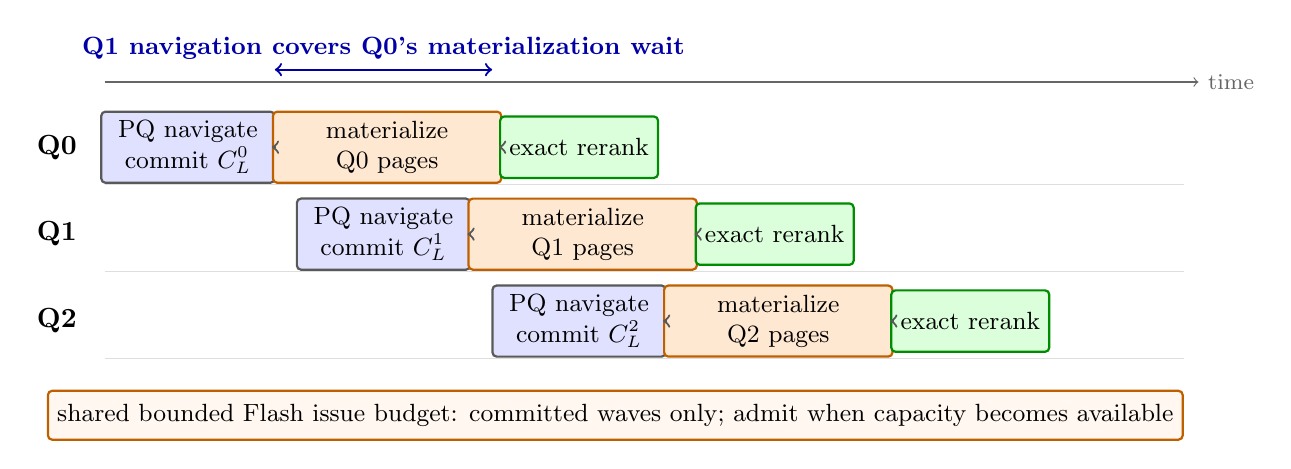
\begin{tikzpicture}[
  x=0.92cm,y=0.92cm,
  font=\small,
  lane/.style={font=\bfseries,anchor=east},
  stage/.style={draw=black!65,thick,rounded corners=1.5pt,
                minimum height=0.78cm,align=center,font=\small},
  nav/.style={stage,fill=blue!12},
  materialize/.style={stage,fill=orange!18,draw=orange!75!black},
  rank/.style={stage,fill=green!14,draw=green!55!black},
  flow/.style={->,thick,draw=black!65}
]
  \draw[->,black!60] (1.20,4.95)--(16.30,4.95)
    node[anchor=west,font=\footnotesize] {time};
  \node[font=\small\bfseries,blue!65!black] at (5.05,5.42)
    {Q1 navigation covers Q0's materialization wait};
  \draw[<->,thick,blue!65!black] (3.55,5.12)--(6.55,5.12);

  \node[lane] at (0.95,4.05) {Q0};
  \node[lane] at (0.95,2.85) {Q1};
  \node[lane] at (0.95,1.65) {Q2};
  \foreach \y in {4.05,2.85,1.65}
    \draw[black!13] (1.20,\y-0.52)--(16.10,\y-0.52);

  \node[nav,minimum width=2.20cm] (q0n) at (2.35,4.05)
    {PQ navigate\\commit $C_L^0$};
  \node[materialize,minimum width=2.90cm] (q0m) at (5.10,4.05)
    {materialize\\Q0 pages};
  \node[rank,minimum width=2.00cm] (q0r) at (7.75,4.05)
    {exact rerank};
  \draw[flow] (q0n)--(q0m); \draw[flow] (q0m)--(q0r);

  \node[nav,minimum width=2.20cm] (q1n) at (5.05,2.85)
    {PQ navigate\\commit $C_L^1$};
  \node[materialize,minimum width=2.90cm] (q1m) at (7.80,2.85)
    {materialize\\Q1 pages};
  \node[rank,minimum width=2.00cm] (q1r) at (10.45,2.85)
    {exact rerank};
  \draw[flow] (q1n)--(q1m); \draw[flow] (q1m)--(q1r);

  \node[nav,minimum width=2.20cm] (q2n) at (7.75,1.65)
    {PQ navigate\\commit $C_L^2$};
  \node[materialize,minimum width=2.90cm] (q2m) at (10.50,1.65)
    {materialize\\Q2 pages};
  \node[rank,minimum width=2.00cm] (q2r) at (13.15,1.65)
    {exact rerank};
  \draw[flow] (q2n)--(q2m); \draw[flow] (q2m)--(q2r);

  \node[draw=orange!75!black,thick,rounded corners=1.5pt,fill=orange!6,
        minimum width=11.9cm,minimum height=0.62cm,font=\small]
    at (8.25,0.35)
    {shared bounded Flash issue budget: committed waves only; admit when capacity becomes available};
\end{tikzpicture}
}
  \caption{Continuous batching fills the service-level bubbles left by a
    single precise materialization wave.
    When Q0 waits for its committed pages, Q1 and Q2 contribute navigation,
    Flash materialization, or reranking under a bounded in-flight budget.
    Each query still crosses its own materialization barrier before reranking,
    so scheduling changes timing but not search semantics.}
  \Description{Three query timelines overlap host-side PQ navigation,
    bounded asynchronous Flash materialization, and exact reranking.  Each
    query reranks only after its own committed pages become resident.}
  \label{fig:design-pipe}
\end{figure*}

\subsection{D5: Observability}
\label{sec:d5}

Every experiment in~\S\ref{sec:eval} is required to report hide counters first: fraction of full-precision scores whose bytes were already in the window (\texttt{score\_from\_window}), critical-path NAND wait (\texttt{crit\_wait\_ns}), and device-fill/wall overlap, then QPS at the iso-recall floor.
Prefetch efficiency is reported as page precision, vector-slot utilization, and extent utilization; a page touched once is not evidence that all of its payload was useful.
QPS without those counters is not a hide result.

\paragraph{What we refuse to hide.}
If a module cannot move \texttt{crit\_wait\_ns} or \texttt{score\_from\_window} in an ablation, it is removed from the contribution list rather than kept as decoration.
An LFU hot set that raises hit rate and drops QPS is already in that bin.

% =============================================================================
% §5 Implementation  — Target: 0.5 page. Disclose what is and is not measured.
% =============================================================================
\section{Implementation}
\label{sec:impl}

\sys{} is a userspace beam search with the adjacency graph and 64-byte PQ codes in host DRAM and full-precision vectors mapped from \texttt{/dev/vmem0}.
The host completes PQ navigation, commits the $L$ rerank candidates, maps them through an ID-to-slot table, and removes resident and duplicate 4\,KiB pages.
The remaining pages form one \texttt{PREFETCH\_BATCH} wave; dense short runs may include bounded holes, and \texttt{PageCopyPool} installs completed pages into DramWindow before full-precision MIPS reranking.
The explicit residency barrier leaves materialization wait on the query path, but prevents the subsequent scoring loads from triggering Flash faults.

\paragraph{What we measure (2026-08-30, \texttt{gpu01}).}
Kernel \texttt{6.18.0-rc5}.
FPGA Altera \texttt{0000:15:00.0} bound to \texttt{ntcx}/\texttt{mem2nvme} (32\,GiB BAR).
NAND I/O goes through \texttt{nvmex} on \texttt{0000:d9:00.0} ($\rightarrow$ \texttt{/dev/nvme4n1}, Dell CD8P 1.92\,TB).
Userspace \texttt{/dev/vmem0} is \texttt{vmem\_sw}: 28\,GiB logical RAM map, 4\,GiB device cache, 2\,MiB stripe.
HPS registers return \texttt{-EOPNOTSUPP}; stores to the BAR read back as \texttt{0xff}.
Hardware \texttt{vmem.ko} implements \texttt{PREFETCH\_BATCH} but is \textbf{not} the measured path.
CXL-DRAM DAX is absent; DramWindow is anonymous pages bound to NUMA node~1.

\paragraph{What is implemented.}
P0 demand access and P3 committed-candidate materialization; host graph and PQ-64 navigation; \texttt{PREFETCH\_BATCH}; co-use/extent layout with an ID-to-slot map; and the iso-recall $L$ picker.
Entry subgraph $\le$32\,MiB is pinned.
A shared LFU hot set was prototyped and \emph{lost} QPS on the warm protocol; we do not ship it as a result.

\paragraph{What is not implemented, and is not claimed.}
Product CXL.mem SSD; HPS fill of the FPGA BAR; Shared FAM; a 160\,GB/s DRAM--SSD engine; closed-loop F9 miss-chop; multi-thread shared-window speedup.
DiskANN PQ-off is never placed on the PQ-on line.

\paragraph{Prototype scale.}
The serving binary is a single translation unit plus small headers on top of the CXAN layout.
The software CXL-SSD path is the out-of-tree \texttt{vmem\_sw} driver.
A log header that omits kernel, BDF, and \texttt{vmem\_sw} vs.\ \texttt{vmem.ko} is an invalid row.

% =============================================================================
% §6 Evaluation  — Route A full matrix. Target: 2.6--3.0 pages.
% 4.5/5 bar: lead with the money plot; iso-recall everywhere; ablate every
% claimed module; name cons; fair DiskANN protocol.
% 填写: 按 caption 合同换图，不要为了更好看改坐标含义。
% =============================================================================
\section{Evaluation}
\label{sec:eval}

We answer five questions:

\begin{enumerate}
  \item[\textbf{Q1}] Does naive CXL-SSD graph ANNS fail in the ways
    \S\ref{sec:motivation} claimed?
  \item[\textbf{Q2}] At iso-recall, does \sys{} move FP scoring off the
    NAND critical path (hide), and what QPS remains vs.\ demand and vs.\
    an in-window oracle?
  \item[\textbf{Q3}] Which module (graph-in-host, bounded install,
    prefetch/\texttt{cont}, page-bin) moves \emph{hide} (critical-path
    wait, score-from-window), not only QPS?
  \item[\textbf{Q4}] Does hide appear only after warmup (service hide),
    or also on a true-cold reload?
  \item[\textbf{Q5}] What remains vs.\ an in-window oracle and vs.\
    PipeANN, and is the residual honest?
\end{enumerate}

\subsection{Setup}
\label{sec:eval-setup}

\begin{table}[t]
  \caption{Locked evaluation platform (2026-08-30, \texttt{gpu01}).}
  \label{tab:setup}
  \small
  \begin{tabular}{@{}ll@{}}
    \toprule
    Item & Configuration \\
    \midrule
    Host CPU / DRAM     & dual-socket Xeon, $\sim$64+64\,GiB host DRAM \\
    CXL-DRAM window     & \textbf{absent}; 1\,GiB DramWindow $=$ \texttt{mbind} node~1 \\
    CXL-SSD             & FPGA \texttt{nvmex}+CD8P; \texttt{/dev/vmem0}=\texttt{vmem\_sw} \\
    Window / cache      & 1\,GiB host window, 4\,GiB \texttt{vmem\_sw} cache \\
    Block-SSD baseline  & PipeANN on \texttt{/mnt/disk0} (\texttt{nvme0n1}), PQ on \\
    Primary corpus      & Text2Image-10M, 200-d, MIPS \\
    Sensitivity         & packed vs.\ page-bin; $L$ picker \\
    Index               & Vamana $R{=}32$, oneshot FP (no PQ nav on serving) \\
    Target quality      & recall@10 $\ge 0.92$ (picker chose $L{=}400$) \\
    Protocol            & cold: \texttt{rmmod} \texttt{vmem\_sw} until \texttt{cache\_used}${}=0$ \\
    \bottomrule
  \end{tabular}
\end{table}

Table~\ref{tab:setup} is the locked configuration. The primary metric is
\emph{iso-recall QPS} (and p99) at a stated recall@$k$ floor. We always
report NAND reads, promote bytes, and the three-level hit breakdown.
A run that does not declare cold vs.\ warm is discarded: the window is
small enough that accidental warm-up invents speedups.

\paragraph{Baselines.}
(1)~\textbf{Demand:} CXL-SSD load/store, no promote.
(2)~\textbf{Page:} 16\,KB admission.
(3)~\textbf{Sync-2hop:} the F3 policy.
(4)~\textbf{Static-wide:} large beam, no controller.
(5)~\textbf{Miss-chop:} cut beam on instantaneous miss (the F9 policy).
(6)~\textbf{DiskANN/PipeANN:} official block path, same machine, same
corpus, same recall floor; PQ on unless a figure is labeled
\texttt{--no\_pq\_nav}.
(7)~\textbf{Oracle-in-window:} pin the measured working set in the
1\,GiB window, then search with no SSD fills (the hide upper bound).
This is not DiskANN.

We never present a home-grown \texttt{O\_DIRECT} reader as ``DiskANN.''

\subsection{Q1: Naive CXL-SSD fails}
\label{sec:eval-mot}

Figure~\ref{fig:mot-cliff}--\ref{fig:mot-bubbles} are reproduced on the
evaluation machine under the Table~\ref{tab:setup} protocol so that
Design and Evaluation share one dataset. We expect the same qualitative
shape: a two-order cliff, page admission and blind prefetch losing to
demand, beam cooling the set, and blocking load/store stuck near
QD$\approx 1$. If a finding does not reproduce, it is dropped from the
intro, not explained away in a footnote.

\subsection{Q2: End-to-end iso-recall (the money plot)}
\label{sec:eval-main}

\begin{figure*}[t]
  \centering
  \phbox{0.98\textwidth}{4.0cm}{%
    Fig.~9 money plot (hide first):\\
    stacked \texttt{crit\_wait} vs.\ compute at iso-recall;\\
    twin axis QPS. Lines: Demand, P3 packed, P3 pagebin,\\
    $-$prefetch, oracle-in-window, PipeANN $T{=}1$.}
  \caption{Hide at the primary recall floor. The money plot is
    critical-path NAND wait, not QPS alone. \sys{} passes only if
    \texttt{crit\_wait} approaches the in-window oracle. QPS vs.\
    PipeANN is a named residual (oneshot FP vs.\ PQ navigation).
    Until hide counters pass we write ``gap to demand,'' not
    ``search cannot see flash.''}
  \Description{Recall versus QPS for the proposed system and baselines.}
  \label{fig:eval-main}
\end{figure*}

\begin{table*}[t]
  \caption{True-cold T2I-10M, $L{=}400$, $nq{=}100$, seed 42, oneshot FP.
    Hide cells (\texttt{crit\_wait}, score-from-window) stay \ph{} until
    the runtime split. NAND/promote columns stay \ph{} until remeasured.}
  \label{tab:eval-main}
  \small
  \setlength{\tabcolsep}{5pt}
  \begin{tabular*}{\textwidth}{@{\extracolsep{\fill}}lrrrrrr@{}}
    \toprule
    System & Recall@10 & QPS & p99 ($\mu$s) & NAND reads/q & Promote B/q & Host DRAM \\
    \midrule
    Demand CXL-SSD (P0) & 0.944 & 1.64 & $1.3{\times}10^{6}$ & \ph & \ph & 1\,GiB win. \\
    Page admission     & \ph & \ph & \ph & \ph & \ph & \ph \\
    Sync 2-hop         & \ph & \ph & \ph & \ph & \ph & \ph \\
    Static wide beam   & \ph & \ph & \ph & \ph & \ph & \ph \\
    Miss-chop beam     & \ph & \ph & \ph & \ph & \ph & \ph \\
    DiskANN (PQ on)    & \ph & \ph & \ph & \ph & --- & \ph \\
    PipeANN pipe T=1   & 0.925 & 57.6 & $1.7{\times}10^{4}$ & \ph & --- & PQ nav \\
    Oracle host DRAM ($nq{=}20$) & 0.950 & 66.5 & $4.8{\times}10^{4}$ & 0 & --- & 9.6\,GiB pop. \\
    Oracle 1\,GiB window ($nq{=}20$) & 0.925 & 85.8 & $1.5{\times}10^{4}$ & 0 & --- & WS pinned \\
    \textbf{\sys{} hide packed} ($nq{=}20$) & 0.930 & 24.67 & $5.7{\times}10^{4}$ & \ph & 100\% win & 1\,GiB \\
    \textbf{\sys{} hide pagebin} ($nq{=}20$, $L{=}400$) & 0.940 & 50.25 & $2.7{\times}10^{4}$ & \ph & 100\% win & 1\,GiB \\
    \textbf{\sys{} hide pagebin} ($nq{=}100$, $L{=}400$) & 0.933 & 49.25 & $3.6{\times}10^{4}$ & \ph & 100\% win & 1\,GiB \\
    \textbf{\sys{} P3 packed} ($nq{=}100$, pre-hide) & 0.944 & 4.08 & $2.4{\times}10^{5}$ & \ph & \ph & 1\,GiB \\
    \textbf{\sys{} P3 pagebin} ($nq{=}100$, pre-hide) & 0.932 & 5.35 & $1.9{\times}10^{5}$ & \ph & \ph & 1\,GiB \\
    \bottomrule
  \end{tabular*}\\[2pt]
  {\footnotesize \phnote}
\end{table*}

Figure~\ref{fig:eval-main} and Table~\ref{tab:eval-main} are the
submission's main result. On the 2026-08-30 true-cold T2I-10M boot
(clock alloc, miss-only, expand-bundle pages),
hide pagebin is $50.25$ QPS at $nq{=}20$ and $49.25$ at $nq{=}100$
($L{=}400$, recall@10 $\ge 0.92$, \texttt{from\_win}${}=100\%$, bounce${}=0$,
in-page slot-use $100\%$ with no extra scores). Neighbors of one expand
share seven sequential pages; we score only those neighbors. Star-BFS
pagebin without the bundle is $25\%$ slot-use (one of five). Real NVMe
occupancy is sectors-read$\times$512 over the timed window over the
isolated random \texttt{PREFETCH\_BATCH} peak ($1.560$\,GB/s), not
``a fill is in flight.'' One query is $0.600/1.560=38.5\%$; four
concurrent queries (private $512$\,MiB windows, $nq{=}100$) reach
$1.027/1.560=65.8\%$ at $87.21$ QPS---the useful-only ceiling
($\approx 12$\,MB/q $\times 87$ QPS $\approx 1.04$\,GB/s). That is
score-path hide; single-query service hide vs.\ the in-window oracle
($85.8$ QPS) is $50.25/85.8\approx 0.59\times$. QPS vs.\ PipeANN (57.6
at $L{=}2000$, PQ on, $T{=}1$) stays a named residual---oneshot FP vs.\
PQ navigation, not a hidden bar. We write the residual as a gap to the
oracle, not ``search cannot see flash.''

\subsection{Q3: Each module is necessary}
\label{sec:eval-ablate}

\begin{figure*}[t]
  \centering
  \phbox{0.98\textwidth}{3.6cm}{%
    Fig.~10 placeholder --- two panels:\\
    (a)~leave-one-out \emph{hide} (crit-wait, score-from-window) and QPS
    (full vs.\ $-$promote $-$prefetch $-$pagebin $-$graph-in-DRAM);
    do not plot $-$LFU-hotset as a loss;\\
    (b)~promote-byte / hot-set-fraction Pareto (QPS vs.\ budget).}
  \caption{Ablation and budget Pareto. Removing any contributed module
    must move the main metric. The Pareto must show a bounded sweet
    spot, not ``more cache is always better.''
    \textbf{Fill-in:} same recall floor as Figure~\ref{fig:eval-main}.}
  \Description{Bar ablation and a Pareto curve of cache/promote budget.}
  \label{fig:eval-ablate}
\end{figure*}

\begin{table}[t]
  \caption{Leave-one-out at the primary recall floor.}
  \label{tab:ablate}
  \small
  \begin{tabular}{@{}lrrr@{}}
    \toprule
    Variant & QPS & \texttt{crit\_wait} & From-win.\\
    \midrule
    Full \sys{} (pagebin)    & 5.35 & \ph & 34\% hit \\
    $-$ page-bin (packed)    & 4.08 & \ph & 3.1\% hit \\
    $-$ \texttt{PREFETCH\_BATCH} & \ph & \ph & must fail hide \\
    $-$ graph-in-host        & \ph & \ph & \ph \\
    $-$ bounded \texttt{install\_top} & \ph & \ph & \ph \\
    Demand only (P0)         & 1.64 & NAND-class & 1.0\% \\
    LFU hot set (void)       & --- & --- & warm QPS collapsed \\
    \bottomrule
  \end{tabular}\\[2pt]
  {\footnotesize \phnote}
\end{table}

Figure~\ref{fig:eval-ablate} and Table~\ref{tab:ablate} are the
falsifiability test for contribution~3. We also sweep promote $M$ and
hot-set fraction to show the F3 lesson in a positive form: there is a
budget at which precision and QPS peak, and past it they fall.

\subsection{Q4: Cold hide versus service hide}
\label{sec:eval-scale}

\begin{figure}[t]
  \centering
  \phbox{0.98\columnwidth}{3.5cm}{%
    Fig.~11 --- cold reload vs.\ 1 discarded warmup:\\
    $y$: \texttt{crit\_wait}, score-from-window, QPS.\\
    If only warm hides, label it service hide.}
  \caption{True-cold (\texttt{vmem\_sw} \texttt{cache\_used}${}=0$) versus
    a discarded warmup then 100 queries. Hide that appears only after
    warmup is a service property, not a cold-start property. Shared-FAM
    provisioning stays a discussion model, not this figure.}
  \Description{Cold versus warm hide metrics on the same index.}
  \label{fig:eval-scale}
\end{figure}

Figure~\ref{fig:eval-scale} is the service question. A production ANNS
process is allowed a discarded warmup; a paper row is not allowed to
confuse that with a true-cold reload. If \texttt{crit\_wait} collapses
only on the warm pass, we say so in the caption and do not migrate the
sentence into~\S\ref{sec:intro}. The one-copy capacity sketch of
\S\ref{sec:background} remains a model; we do not plot it as a measured
Q4.

\subsection{Q5: Losses, overhead, and fairness}
\label{sec:eval-limit}

We report the cases \sys{} loses or looks worse: warm working sets that
already fit the window (async prefetch $\approx$ demand); low dimension
where page$\approx$record; the residual gap to PQ-navigated DiskANN;
and software-proxy artifacts (global cache lock, QD ceiling). Host-DRAM
consumed by the graph and PQ is a cost, not a footnote. CPU is reported
because DiskANN on this class of machine is I/O-bound, not CPU-bound;
if \sys{} becomes CPU-bound we say so.

\paragraph{Takeaway.}
Q2--Q4 must be answerable from hide counters, not from QPS prose. If the
money plot needs a verbal caveat that changes the claim, the claim in
\S\ref{sec:intro} is the thing to change.

% =============================================================================
% §7 Related Work  — Target: 0.7 page + Table 5.
% 4.5/5 bar: 4 sentences per neighbor (where data lives, slow path, delay
% scale, one-line difference). No "they also do ANNS."
% 填写: 把 Anonymous bib 换成正式引用；不要扩大 “first” 范围。
% =============================================================================
\section{Related Work}
\label{sec:related}

Table~\ref{tab:related} is the comparison we want a reviewer to use.
Prose below only records the one-line difference; it does not repeat the background.

\begin{table}[t]
  \caption{Closest systems and their defining distinction.}
  \label{tab:related}
  \scriptsize
  \setlength{\tabcolsep}{2.5pt}
  \begin{tabular}{@{}p{0.25\columnwidth}p{0.25\columnwidth}p{0.43\columnwidth}@{}}
    \toprule
    System & Slow tier & Primary distinction \\
    \midrule
    DiskANN / PipeANN & block SSD & PQ navigation + async block I/O \\
    Second-Tier / FaTRQ & far memory & coarse/fine far reads \\
    CXL-ANNS / Cosmos & CXL DRAM / PNM & memory latency or compute offload \\
    CXL-SSD hardware & NAND + window & generic memory-semantic access \\
    \textbf{\sys{}} & \textbf{CXL-SSD} & \textbf{committed pages + cross-query overlap} \\
    \bottomrule
  \end{tabular}
\end{table}

\paragraph{Block-SSD ANNS}
DiskANN, FreshDiskANN, and PipeANN optimize PQ navigation and I/O overlap on block devices~\cite{diskann,freshdiskann,pipeann}; SPANN and Starling explore hybrid or disk-resident layouts~\cite{spann,starling}.
SPFresh, Filtered-DiskANN, and Milvus extend this space to updates, filters, and serving~\cite{spfresh,filtereddiskann,milvus}.
Unlike an I/O scheduler, \sys{} manages a memory-semantic window and the committed vector pages required before exact reranking.

\paragraph{CXL-DRAM and near-memory ANNS}
CXL-ANNS, Cosmos, and second-tier/residual designs assume a DRAM- or NVM-priced far tier~\cite{cxlanns,cosmos,secondtier,fatrq,hm-ann}; CXL-aware vector-database restructuring makes the same memory-class assumption~\cite{bauhaus}.
Their $\sim$100\,ns policies do not address tens-of-microseconds NAND behind a polluted window (F3), and \sys{} does not require near-memory compute.

\paragraph{Far-memory runtimes and CXL tiering}
Remote paging and application-integrated runtimes manage far capacity through paging, isolation, and prefetch~\cite{infiniswap,canvas,aifm,leap,rethinkingruntimes}; CXL tiering places hot pages across DRAM-class tiers~\cite{tpp,nomad,neomem,memtierscxl,canfarmemory,pond}.
Those policies react to generic locality; \sys{} uses PQ commitment to identify reranking's full-precision payload.

\paragraph{CXL-SSD hardware and generic software}
DirectCXL and memory pooling establish CXL expansion~\cite{directcxl,memorypooling}; CXL-enabled SSD, SkyByte, From-Block-to-Byte, and CMM-H study flash-backed memory~\cite{cxlssd,skybyte,fromblocktobyte,cmmh}.
They do not jointly manage graph-ANNS residency, committed-vector materialization, and cross-query overlap.

% =============================================================================
% §8 Discussion / Limitations
% =============================================================================
\section{Discussion and Limitations}
\label{sec:discuss}

\paragraph{Proxy versus product.}
The measured path is FPGA \texttt{nvmex} plus \texttt{vmem\_sw}, not a shipping CXL.mem SSD.
HPS does not fill the 32\,GiB BAR from the host CPU; we will not relabel that BAR as the evaluated window.
Latency cliffs and QD collapse are still properties of memory-semantic flash.

\paragraph{Hide is the service contract, not a fallback.}
A usable ANNS service on this tier means the scoring thread does not wait on NAND: every full-precision distance is taken from bytes already in the window (\texttt{score\_from\_window}${}=100\%$), and \texttt{crit\_wait\_ns} is DRAM-class.
Graph/PQ live in host DRAM; entry 2-hop is warmed off the timed path; lookahead plus continuous fills keep the next hop resident.
A window miss while scoring is a hide failure we close, not a reason to shrink the claim.

\paragraph{One-copy is a deployment claim, not a result.}
Figure~\ref{fig:eval-scale}b is a provisioning model.
Shared FAM is unmeasured.
Device IOPS remain shared even with one copy.

\paragraph{DiskANN/PipeANN remain the block-path champions.}
PQ navigation plus deep \texttt{aio} avoids most full-precision reads.
\sys{} oneshot-FP on a load/store flash mapping is a different contract.
A $\sim$11$\times$ QPS gap to PipeANN $T{=}1$ at iso-recall is expected and reported.

\paragraph{Hot set and \texttt{install\_all}.}
A 64\,MiB shared LFU set raised hit rate and destroyed QPS (window thrash).
D3 in the paper is entry pin $+$ soft-pin.
True-cold \texttt{install\_all} did not reproduce a historical $\div$5 QPS drop; we report traffic, not a fake collapse.

\paragraph{What would change our mind.}
If HPS makes the FPGA BAR a coherent miss window, we re-measure hide there and keep the same counters.
If hide counters never leave NAND-class wait, contribution~3 shrinks to ``overlap vs.\ demand'' and the intro must not say the host is unaware of CXL-SSD.

% =============================================================================
% §9 Conclusion  — Target: 0.15--0.2 page. Restate opportunity vs. system.
% =============================================================================
\section{Conclusion}
\label{sec:concl}

Graph ANNS has a well-engineered block-SSD path and a well-engineered CXL-DRAM path.
Flash-backed CXL memory is the third deployment point --- flash-priced capacity, a memory-semantic window, and a future one-copy hosting story --- but it is unusable if treated as slow DRAM or as mmap'd DiskANN.
\sys{} is a runtime for that tier: after host-side PQ navigation commits a rerank set, wise prefetch materializes only its missing full-precision vector pages, and continuous batching schedules those precise batches across queries.
The opportunity is the medium; the contribution is separating search information from payload movement so exact scoring reads resident bytes while the remaining materialization wait stays explicit.


\bibliographystyle{ACM-Reference-Format}
\bibliography{refs}

\appendix
% =============================================================================
% Appendix --- does NOT count toward the 11-page limit.
% Reviewers are not required to read this. Put extra sweeps here, not claims
% that the main text needs.
% =============================================================================
\section{Fill-in Checklist}
\label{app:checklist}

Table~\ref{tab:app-checklist} is the author-facing map from each
placeholder to the result file that should replace it. Delete this
appendix before a submission if it is still author notes; or keep a
cleaned artifact appendix after the numbers exist.

\begin{table*}[t]
  \caption{Placeholder $\rightarrow$ intended source. Author notes; not a
    scientific result.}
  \label{tab:app-checklist}
  \small
  \begin{tabular}{@{}llp{0.46\textwidth}@{}}
    \toprule
    Id & Type & Replace with \\
    \midrule
    Fig.~\ref{fig:intro-position} & figure* & 3-column deployment $+$ runtime overlay \\
    Fig.~\ref{fig:bg-cxl} & figure & Measured/proxy CXL-SSD stack \\
    Fig.~\ref{fig:mot-cliff} & figure & Cold / soft / warm latency $+$ search breakdown \\
    Fig.~\ref{fig:mot-pathology} & figure* & Page vs.\ record; prefetch precision; beam sweep \\
    Fig.~\ref{fig:mot-bubbles} & figure & \texttt{sections/fig\_bubbles.tex} or a measured redraw \\
    Tab.~\ref{tab:findings} & table & Headline deltas from MOTIVATION\_FINDINGS \\
    Fig.~\ref{fig:design-arch} & figure* & Implemented component names \\
    Tab.~\ref{tab:placement} & table & Byte counts on the primary corpus \\
    Fig.~\ref{fig:design-promote} & figure & Promote API $+$ default $M$/budget \\
    Fig.~\ref{fig:design-pipe} & figure* & \texttt{cont} $+$ async fill; blocking mmap failure \\
    Tab.~\ref{tab:setup} & table & Locked platform and corpora \\
    Fig.~\ref{fig:eval-main} & figure* & Iso-recall QPS (money plot) \\
    Tab.~\ref{tab:eval-main} & table* & End-to-end row per baseline \\
    Fig.~\ref{fig:eval-ablate} & figure* & Leave-one-out $+$ Pareto \\
    Tab.~\ref{tab:ablate} & table & Leave-one-out numbers \\
    Fig.~\ref{fig:eval-scale} & figure & Scale sweep $+$ provisioning model \\
    Tab.~\ref{tab:related} & table* & Camera-ready citations \\
    \bottomrule
  \end{tabular}
\end{table*}

\section{Artifact Outline}
\label{app:artifact}

An ASPLOS artifact should include: the identity gate for the CXL-SSD
node; scripts that reset the window (cold protocol); the iso-recall
harness; and the exact command lines that produce
Figures~\ref{fig:eval-main}--\ref{fig:eval-scale}. We will not point a
reviewer at an identifiable internal hostname.


\end{document}
